\documentclass[pgmicro,diss,openright,oneside]{iiufrgs}
% Para usar o modelo, deve-se informar o programa e o tipo de documento.
% Programas :
%   * cic       -- Graduação em Ciência da Computação
%   * ecp       -- Graduação em Ciência da Computação
%   * ppgc      -- Programa de Pós Graduação em Computação
%   * pgmigro   -- Programa de Pós Graduação em Microeletrônica
%   
% Tipos de Documento:
%   * tc                -- Trabalhos de Conclusão (apenas cic e ecp)
%   * diss ou mestrado  -- Dissertações de Mestrado (ppgc e pgmicro)
%   * tese ou doutorado -- Teses de Doutorado (ppgc e pgmicro)
%   * ti                -- Trabalho Individual (ppgc e pgmicro)
% 
% Outras Opções:
%   * english    -- para textos em inglês
%   * openright  -- Força início de capítulos em páginas ímpares (padrão da
%                   biblioteca)
%   * oneside    -- Desliga frente-e-verso
%   * nominatalocal -- Lê os dados da nominata do arquivo nominatalocal.def


% Use unicode
\usepackage[utf8]{inputenc}   % pacote para acentuação

% Necessário para incluir figuras
\usepackage{graphicx}           % pacote para importar figuras

\usepackage{color}           % pacote para usar cores no texto

\usepackage{times}              % pacote para usar fonte Adobe Times
% \usepackage{palatino}
% \usepackage{mathptmx}          % p/ usar fonte Adobe Times nas fórmulas

\usepackage[alf,abnt-emphasize=bf]{abntex2cite}	% pacote para usar citações abnt

\usepackage{epigraph}		%pacote para usar epígrafe

%
% Informações gerais
%
\title{Hardware dinâmico para tolerância a falhas em microprocessadores}

\author{Augusto}{Thiago Rider}

\advisor[Prof.~Dr.]{Beck Filho}{Antônio Carlos Schneider}
%\coadvisor[Prof.~Dr.]{Silva}{Fulano da}

% a data deve ser a da defesa; se nao especificada, são gerados
% mes e ano correntes
\date{dezembro}{2015}

% o local de realização do trabalho pode ser especificado (ex. para TCs)
% com o comando \location:
\location{Porto Alegre}{RS}

% itens individuais da nominata podem ser redefinidos com os comandos
% abaixo:
% \renewcommand{\nominataReit}{Prof\textsuperscript{a}.~Wrana Maria Panizzi}
% \renewcommand{\nominataReitname}{Reitora}
% \renewcommand{\nominataPRE}{Prof.~Jos{\'e} Carlos Ferraz Hennemann}
% \renewcommand{\nominataPREname}{Pr{\'o}-Reitor de Ensino}
% \renewcommand{\nominataPRAPG}{Prof\textsuperscript{a}.~Joc{\'e}lia Grazia}
% \renewcommand{\nominataPRAPGname}{Pr{\'o}-Reitora Adjunta de P{\'o}s-Gradua{\c{c}}{\~a}o}
% \renewcommand{\nominataDir}{Prof.~Philippe Olivier Alexandre Navaux}
% \renewcommand{\nominataDirname}{Diretor do Instituto de Inform{\'a}tica}
% \renewcommand{\nominataCoord}{Prof.~Carlos Alberto Heuser}
% \renewcommand{\nominataCoordname}{Coordenador do PPGC}
% \renewcommand{\nominataBibchefe}{Beatriz Regina Bastos Haro}
% \renewcommand{\nominataBibchefename}{Bibliotec{\'a}ria-chefe do Instituto de Inform{\'a}tica}
% \renewcommand{\nominataChefeINA}{Prof.~Jos{\'e} Valdeni de Lima}
% \renewcommand{\nominataChefeINAname}{Chefe do \deptINA}
% \renewcommand{\nominataChefeINT}{Prof.~Leila Ribeiro}
% \renewcommand{\nominataChefeINTname}{Chefe do \deptINT}

% A seguir são apresentados comandos específicos para alguns
% tipos de documentos.

% Relatório de Pesquisa [rp]:
% \rp{123}             % numero do rp
% \financ{CNPq, CAPES} % orgaos financiadores

% Trabalho Individual [ti]:
% \ti{123}     % numero do TI
% \ti[II]{456} % no caso de ser o segundo TI

% Monografias de Especialização [espec]:
% \espec{Redes e Sistemas Distribuídos}      % nome do curso
% \coord[Profa.~Dra.]{Weber}{Taisy da Silva} % coordenador do curso
% \dept{INA}                                 % departamento relacionado

%
% palavras-chave
% iniciar todas com letras minúsculas, exceto no caso de abreviaturas
%
\keyword{Tolerância à Falhas}
\keyword{Detecção de Erros}
\keyword{Hardware Adaptativo}
\keyword{Microprocessadores}

%
% inicio do documento
%
\begin{document}

% folha de rosto
% às vezes é necessário redefinir algum comando logo antes de produzir
% a folha de rosto:
% \renewcommand{\coordname}{Coordenadora do Curso}
\maketitle

% dedicatoria
\clearpage
\begin{flushright}
\mbox{}\vfill
{\sffamily\itshape
``Logic will get you from A to B. \\
Imagination will take you everywhere.''\\}
--- \textsc{Albert Einstein}
\end{flushright}

% agradecimentos
\chapter*{Agradecimentos}
Agradeço ao \LaTeX\ por não ter vírus de macro\ldots



% resumo na língua do documento
\begin{abstract}
Com a evolução dos processos de fabricação de dispositivos eletrônicos, um fenômeno já conhecido passa a afetar ainda mais os circuitos: trata-se do fenômeno da radiação cósmica. Logo, ao tentar se utilizar circuitos no meio espacial, é necessária a devida adaptação com técnicas especializadas para mitigar falhas que podem levar a efeitos catastróficos e arruinar missões espaciais. Ao passar dos anos, muitas técnicas foram desenvolvidas em diferentes níveis: hardware, software ou híbridas. A suscetibilidade dos circuitos a radiação está ligada a maior integração, que faz com que os transistores sejam cada vez mais diminutos. Com as chaves menores, a chance de uma partícula afetar um ou mais dispositivos é muito maior. O aumento da frequência de operação também ocupa lugar nessa problemática, haja visto que com um intervalo mais curto entre as bordas de relógio, aumenta-se a probabilidade de um pulso espúrio ser capturado pela lógica. A complexidade e tamanho dos circuitos também ficaram maiores e grande parte dos sistemas é microprocessado, levando a um interesse ainda maior de proteger essa classe de sistemas. Este trabalho visa implementar em hardware diversas técnicas de detecção de erros, com o objetivo de proteger processadores contra falhas transientes, propondo um  módulo especializado, capaz de atuar dinamicamente selecionando uma técnica, levando em consideração a melhor relação entre o custo do tempo de execução e a taxa de detecção de erros. Tem relevância no contexto de uso de sistemas micro processados em ambientes hostis cuja exposição à radiação ou ainda, influência eletromagnética podem causar efeitos inesperados no comportamento do circuito.
\end{abstract}

% resumo na outra língua
% como parametros devem ser passados o titulo e as palavras-chave
% na outra língua, separadas por vírgulas
\begin{englishabstract}{Dynamic hardware for fault tolerance in microprocessors}{Fault Tolerance,Error Detection,Adaptative Hardware,Microprocessors}
With the development of electronic devices manufacturing processes, an already known phenomenon becomes even more affect the circuits: it is the phenomenon of cosmic radiation. Then when you try to use circuits in the space environment, appropriate adjustment is required with specialized techniques to mitigate failures that can lead to catastrophic effects and ruin space missions. Over the years, many techniques have been developed at different levels: hardware, software or hybrid. The susceptibility of circuits radiation is linked to greater integration, which makes the transistors are increasingly tiny. With the minor keys, the chance of a particle affect one or more devices is much higher. Increasing the frequency of operation also takes place on these problems, there is seen that with a shorter interval between the clock edges, increases the likelihood of a spurious pulse is captured by logic. The complexity and size of the circuits were also larger and much of the microprocessor systems is leading to an even greater interest in protecting this class of systems. This work aims to implement in hardware several error detection techniques, in order to protect against transient faults processors, offering a specialized module, able to act dynamically selecting a technique, taking into account the best ratio between the cost of run time and error detection rate. Has relevance in micro systems use context processed in hostile environments where exposure to radiation or, electromagnetic influence can cause unexpected effects on circuit behavior.
\end{englishabstract}

% lista de abreviaturas e siglas
% o parametro deve ser a abreviatura mais longa
\begin{listofabbrv}{SPMD}
        \item[SMP] Symmetric Multi-Processor
        \item[NUMA] Non-Uniform Memory Access
        \item[SIMD] Single Instruction Multiple Data
        \item[SPMD] Single Program Multiple Data
        \item[ABNT] Associação Brasileira de Normas Técnicas
\end{listofabbrv}

% idem para a lista de símbolos
%\begin{listofsymbols}{$\alpha\beta\pi\omega$}
%       \item[$\sum{\frac{a}{b}}$] Somatório do produtório
%       \item[$\alpha\beta\pi\omega$] Fator de inconstância do resultado
%\end{listofsymbols}

% lista de figuras
\listoffigures

% lista de tabelas
\listoftables

% sumario
\tableofcontents

% aqui comeca o texto propriamente dito

% Introducao
\chapter{Introdução}

\epigraph{\sffamily\itshape
``Little by little, one travels far.''}{--- \textsc{J.R.R. Tolkien}}


As prospecções do International Technology Roadmap for Semiconductors (ITRS) preveem que em pouco tempo teremos transistores de menos de meia dezena de nanômetros, além de tecnologias com múltiplos gates(MGT) e isso implica em: menor confiabilidade dos transistores, manifestações de efeitos da radiação ao nível do mar, menores capacitâncias(menores cargas armazenadas), menores margens de ruído e menor consumo.\cite{Massengill2012}

Enquanto a tecnologia avança no sentido da escalabilidade, a radiação e seus efeitos permanecem como um fenômeno prejudicial ao correto funcionamento dos circuitos eletrônicos, afetando ainda mais estes a cada mudança de nó tecnológico. O que antes era foco de atenção quase que exclusivamente no setor aeroespacial, vem a ser preocupação também ao nível do mar.\cite{Massengill2012}

O entendimento de um tipo de evento causado pela radiação, o \textit{Single-Event Upset}(SEU), é reconhecidamente uma das preocupações-chave no que tange a confiabilidade dos circuitos para a tecnologia atual e futura. A natureza deste evento tem origem numa partícula carregada que passa por um dispositivo microeletrônico e ioniza o material pelo caminho percorrido. Ao ocorrer esta ionização, são gerados pares elétron-lacuna. Os portadores livres(elétrons e lacunas) eventualmente serão recombinados. Esta recombinação pode ser evitada em condições apropriadas de operação de um dispositivo, através dos campos elétricos internos. Com isso, um pulso elétrico é gerado, sendo grande o suficiente para interromper o funcionamento normal do dispositivo. Este fenômeno não esta associado a um dano permanente no dispositivo, porém o resultado é um erro num bit. O fenômeno é chamado de \textit{Single-Event Upset}(SEU), ou ainda, \textit{soft error} ou \textit{soft failure}\cite{Tang2003}. Segundo o dicionário de termos usados na área aeroespacial da \citen{Scientific2010}, SEUs são descritos de forma semelhante com a seguinte definição:

\begin{quote}
\emph{\textbf{Single Event Upsets}}: Radiation-induced errors in microelectronic circuits caused when charged particles(usually from the radiation belts or from cosmic rays) lose energy by ionizing the medium through which they pass, leaving behind a wake of electron-hole pairs.
\end{quote}

Nota-se que nesta definição são incluídas possíveis fontes das partículas: cinturões de radiação ou raios cósmicos.

\section{Objetivos}
Este trabalho tem como objetivo principal realizar uma pesquisa e implementação de um hardware adaptativo para tolerância a falhas utilizando técnicas para microprocessadores já consagradas na literatura científica da área.

Para alcançar esta meta principal, o percurso da pesquisa inclui objetivos secundários, sejam eles: 

\begin{itemize}

\item Realizar uma revisão bibliográfica sobre: as técnicas de tolerância a falhas em microprocessadores, as metodologias de verificação de hardware, técnicas de injeção de falhas e sobre o fenômeno da radiação cósmica em circuitos eletrônicos;
\item Solidificar os conhecimentos sobre a arquitetura MIPS através do conhecimento do microprocessador escolhido para o trabalho;
\item Ser capaz de selecionar uma metodologia de verificação de hardware e também de injeção de falhas a ser utilizada em conjunto com o simulador para uma campanha de injeção de falhas;
\item Selecionar algumas técnicas de tolerância a falhas para serem implementadas no hardware;
\item Propor \textit{datapath} e controle para cada técnica de tolerância a falhas selecionada para compôr o hardware;
\item Integrar as técnicas para um funcionamento contínuo do sistema, sendo assim adaptativo às diversas situações do ambiente injetor de falhas.

\end{itemize}

\section{Justificativa}
A avaliação de diversas técnicas de detecção de erros em software, com o objetivo de proteger processadores contra falhas transientes e ainda, a implementação em hardware de forma a atuar dinamicamente selecionando qual a melhor técnica tem relevância no contexto de uso de sistemas microprocessados em ambientes hostis cuja exposição à radiação ou ainda, influência eletromagnética podem causar efeitos inesperados no comportamento do circuito, aproveitando o menor custo computacional disponível para uma dada taxa de erros detectados.

\section{Expectativas}
Espera-se que com o hardware desenvolvido e o ambiente injetor de falhas seja possível comparar o custo, em tempo de processamento adicional, necessário para a execução de um mesmo algoritmo aplicando-se cada técnica disponível no módulo. Para que isso seja possível, um dicionário de dados e uma análise da cobertura de falhas devem ser explorados ao decorrer da campanha de injeção de falhas. 

É possível que com os resultados decorrentes da injeção de falhas em diversos pontos do processador sejam utilizados para realizar uma análise dos pontos mais suscetíveis a falhas no projeto do processador. 

Além do tempo de processamento, é esperado obter um tamanho em portas lógicas para este hardware, já que é uma métrica interessante para efeitos comparativos com o processador em si. No caso de um implementação no mesmo \textit{die}, é importante saber qual o espaço adicional que o módulo ocuparia.

% Capítulo 2
\chapter{Contexto da Pesquisa}
\section{O processador miniMIPS}
\section{A Origem de tudo: As 3 causas de problemas com a radiação cósmica}
\section{\textit{Background} de tolerância a falhas}
	\subsection{Radiação e Efeitos}
	\subsection{Eletrônica, SEUs e SETs}
	\subsection{Métricas para avaliar suscetibilidade dos circuitos}
	\subsection{Técnicas de detecção de erros em processadores}
	\subsection{Técnicas de mitigação para SEUs e SETs em processadores}

% Capítulo 3
\chapter{Robustecimento de Processadores Contra Efeitos da Radiação Cósmica}

\epigraph{\sffamily\itshape
``The scientific man does not aim at an immediate result. His duty is to lay the foundation for those who are to come, and point the way.''}{--- \textsc{Nikola Tesla}}



\section{Proteções em hardware}
\section{Proteções em software}
\section{Fragilidades das proteções em hardware e software}

% Capítulo 4
\chapter{Hardware Adaptativo para Tolerância a Falhas}
\section{Porque adaptativo?}
\section{Arquitetura proposta}
	\subsection{Máquina de estados para a técnica EDDI}
	\subsection{Máquina de estados para a técnica 2}
	\subsection{Máquina de estados para a técnica 3}
\section{Metodologia de verificação adaptada a uma campanha de injeção de falhas}
\subsection{Metodologia de Verificação Universal}
\subsection{Experimentos de injeção de falhas em simulação}
\subsubsection{Biblioteca de injeção de falhas usando VPI}
\subsubsection{Premissas ao se injetar falhas}
\section{Integrando as máquinas de estados propostas}


% Capítulo 5
\chapter{Análise e Resultados da Pesquisa}
\section{Casos de teste usando o módulo RFTAH}


% Conclusão
\chapter{Conclusão}

\epigraph{\sffamily\itshape
``One never notices what has been done; one can only see what remains to be done.''}{--- \textsc{Marie Curie}}

Concluindo...

	\section{Trabalhos Futuros}

A melhora disso ou daquilo.... como trabalho futuro.

Uma nova implementação da técnica XYZ... também é justificada por tal e tal motivo.

A exploração em outra arquitetura de microprocessador tal e tal ajudaria nisso naquilo ou naquilo outro...



% Exemplos de Formatação
\chapter{Exemplos de Uso do \LaTeX}
No início dos tempos, Donald E. Knuth criou o \TeX. Algum tempo depois, Leslie Lamport criou o \LaTeX. Graças a eles, não somos obrigados a usar o Word nem o LibreOffice.

\section{Figuras e tabelas}

Esta seção faz referência às Figuras~\ref{fig:estrutura},~\ref{fig:ex1} e~\ref{fig:ex2}, a título de exemplo. A primeira figura apresenta a estrutura de uma figura. A \emph{descrição} deve aparecer \textbf{acima} da figura. Abaixo da figura, deve ser indicado a origem da imagem, mesmo se essa for apenas os autores do texto. Segundo \cite{Ziade2004}, blah blhah blah...
Os artigos de \cite{Azambuja2010,Abate2008,Al-Yamani,Alkhalifa1999} servem de exemplos disso, daquilo e daquilo outro...

A Figura~\ref{fig:ex1} representa o caso mais comum, onde a figura propriamente dita é importada de um arquivo (neste exemplo em formato \texttt{eps} ou \texttt{pdf}. Veja a seção \ref{sec:fig_format}). A Figura~\ref{fig:ex2} exemplifica o uso do environment \texttt{picture}, para desenhar usando o próprio~\LaTeX.

\begin{figure}[h]
    \caption{Descrição da Figura deve ir no topo}
    \begin{center}
        % Aqui vai um includegraphics , um picture environment ou qualquer
        % outro comando necessário para incorporar o formato de imagem
        % utilizado.
        \begin{picture}(100,100)
                \put(0,0){\line(0,1){100}}
                \put(0,0){\line(1,0){100}}
                \put(100,100){\line(0,-1){100}}
                \put(100,100){\line(-1,0){100}}
                \put(10,50){Uma Imagem}
        \end{picture}
    \end{center}
    \label{fig:estrutura}
    \legend{Fonte: Os Autores}
\end{figure}

\begin{figure}
    \caption{Exemplo de figura importada de um arquivo e também exemplo de caption muito grande que ocupa mais de uma linha na Lista~de~Figuras}
    \centerline{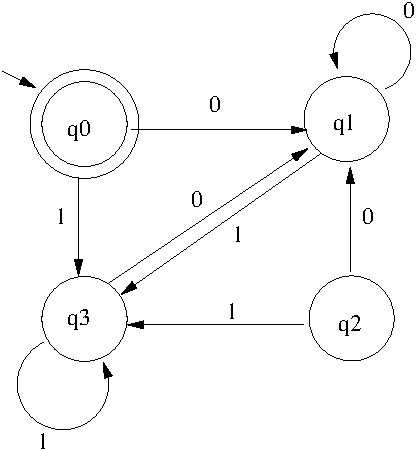
\includegraphics[width=8em]{fig}}
    \legend{Fonte: Os Autores}
    \label{fig:ex1}
\end{figure}

% o `[h]' abaixo é um parâmetro opcional que sugere que o LaTeX coloque a
% figura exatamente neste ponto do texto. Somente preocupe-se com esse tipo
% de formatação quando o texto estiver completamente pronto (uma frase a mais
% pode fazer o LaTeX mudar completamente de idéia sobre onde colocar as
% figuras e tabelas)
%\begin{figure}[h]
\begin{figure}
    \caption{Exemplo de figura desenhada com o environment \texttt{picture}.}
    \begin{center}
        \setlength{\unitlength}{.1em}
        \begin{picture}(100,100)
                \put(20,20){\circle{20}}
                \put(20,20){\small\makebox(0,0){a}}
                \put(80,80){\circle{20}}
                \put(80,80){\small\makebox(0,0){b}}
                \put(28,28){\vector(1,1){44}}
        \end{picture}
    \end{center}
    \legend{Fonte: Os Autores}
    \label{fig:ex2}
\end{figure}

Tabelas são construídas com praticamente os mesmos comandos. Ver a tabela \ref{tbl:ex1}.

\begin{table}[h]
    \caption{Uma tabela de Exemplo}
    \begin{center}
        \begin{tabular}{c|c|p{5cm}}
            \textit{Col 1}  &   \textit{Col 2}  &   \textit{Col 3} \\
            \hline
            \hline
            Val 1           &   Val 2           & Esta coluna funciona como um parágrafo, tendo uma margem definida em 5cm. Quebras de linha funcionam como em qualquer parágrafo do tex. \\
            Valor Longo     & Val 2             & Val 3 \\
            \hline
        \end{tabular}
    \end{center}
    \legend{Fonte: Os Autores}
    \label{tbl:ex1}
\end{table}

\subsection{Formato de Figuras}
\label{sec:fig_format}

O LaTeX permite utilizar vários formatos de figuras, entre eles \emph{eps}, \emph{pdf}, \emph{jpeg} e \emph{png}. Programas de diagramação como Inkscape (e mesmo LibreOffice) permitem gerar arquivos de imagens vetoriais que podem ser utilizados pelo LaTeX sem dificuldade. Pacotes externos permitem utilizar SVG e outros formatos.

Dia e xfig são programas utilizados por dinossauros para gerar figuras vetoriais. Se possível, evite-os.

\subsection{Classificação dos etc.}

O formato adotado pela ABNT prevê apenas três níveis (capítulo, seção e subseção). Assim, \texttt{\char'134subsubsection} não é aconselhado.

\section{Sobre as referências bibliográficas}

A classe \emph{iiufrgs} faz uso do pacote \emph{abnTeX2} com algumas alterações
feitas por Sandro Rama Fiorini. Culpe ele se algo der errado. Agradeça a ele
pelo que der certo. As modificações dão uma camada de tinta NATBIB-style,
já que o abntex2 usa uns comandos de citação feitos para alienígenas de 5 braços 
wtf. Exemplos de citação:

\begin{itemize}

	\item \emph{cite}: Unicórnios são verdes \cite{Nicolaidis2011};
	\item \emph{citep}:Unicórnios são verdes \citep{SimondDavidmann2014};
	\item \emph{citet}: Segundo \citet{Nicolaidis2011}, unicórnios são verdes.
	\item \emph{citen or citenum}: Segundo \citen{Rebaudengo2004}, unicórnios são verdes.
	\item \emph{citeauthor e citeyearpar}: Segundo artigos de \citeauthor{Alkhalifa1999}, unicórnios são verdes \citeyear{Nicolaidis2011}.

\end{itemize}

O estilo abnt fornecido antigamente pelo UTUG não é mais recomendado, pois não
produz saída de acordo com as exigências da biblioteca.

Recomenda-se o uso de bibtex para gerenciar as referências (veja o arquivo
biblio.bib).


% referencias
% aqui será usado o environment padrao `thebibliography'; porém, sugere-se
% seriamente o uso de BibTeX e do estilo abnt.bst (veja na página do
% UTUG)
%
% observe também o estilo meio estranho de alguns labels; isso é
% devido ao uso do pacote `natbib', que permite fazer citações de
% autores, ano, e diversas combinações desses

\bibliographystyle{abntex2-alf}
\bibliography{biblio}

\appendix

\chapter{CONTRIBUIÇÕES}

\end{document}